\pagestyle{plain}
\section*{Der Skistock zum Messen der Hangneigung}
\section*{Anleitung}


\begin{wrapfigure}{r}{0.42\textwidth}
\vspace{-\intextsep}
\centering
\begin{minipage}{0.39\textwidth}
\vspace{0pt}
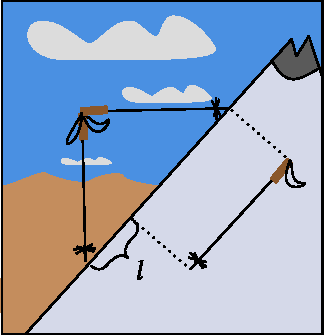
\includegraphics{./Bilder/AllgemeinerAufbau.pdf}

\end{minipage}%
\end{wrapfigure}
Zunächst wird die Länge des Skistocks in die Fallrichtung markiert.Danach werden die beiden Skistöcke in einer Hand gehalten.
 Einer der beiden Skistöcke wird an die obere Markierung in den Schnee gesteckt und der weitere Skistock wird hängen gelassen. Nun bewegt man die Hand so, dass der zweite Skistock unterhalb des ersten entlang der Falllinie den Hang berührt. Im Bild ist der Querschnitt zu sehen. Die länge $l$ misst nun, wie viele $\unit{cm}$ der zweite stock unterhalb der Markierung den Hang berührt. Die Faustregel zur berechnung der Hangneigun ist nun die folgende: 

 \begin{equation*}
    \text{Hangneigung}=30^{\circ}+\frac{10}{3}l
 \end{equation*}
 Oder in Worten: 
 Trifft der zweite Stock die untere Markierung so hat der Hang $30 ^{\circ}$. Für je $10 \unit{cm}$.
  Abstand müssen wir $3^{\circ}$ hinzunehmen. Ist $l$ negativ, beziwhungsweist trifft der zweite stock oberhalb der unteren Markierung den Hang, so müssen wir für jeh $10\unit{cm}$ $3^{\circ}$ abziehen.
  \section*{Begründung}
  \subsection*{Der einfache Fall}
  \begin{wrapfigure}{l}{0.4\textwidth}
  \vspace{-\intextsep}
  \centering
  \begin{minipage}{0.39\textwidth}
  \vspace{0pt}
   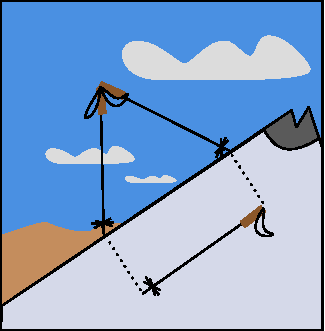
\includegraphics{./Bilder/AufbauEinfacherFall.pdf}
  \end{minipage}%  
  \end{wrapfigure}
  Wir beginnen mit dem Einfachsten Fall, falls $l=0$ ist, d.h. falls der zweite Stock die untere Markierung trifft.
  Nun ist ein gleichseitiges Dreieck auch gleichwinklig. D.h. alle Innenwinkel sind identisch. Das lässt sich leicht aus den Kongruenzsätzen herleiten: Ist ein gleichseitiges Dreieck mit den Eckpunkten $A.B,C$ gegeben, dass wir im folgenden $\Delta ABC$ nennen, so ist dieses aufgrund des Kongruenzsatzes SSS (Seite Seite Seite) kongruent zu dem Dreieck $\Delta BCA$ mit den Ecken $B,C,A$. Damit sind auch die drei Winkel gleich, weshalb der Innenwinkel in $B$, dem Innenwinkel in $A$ gleicht. Analog erhält man auch das der Innenwinkel in $C$ dem in $A$ gleicht und somit alle identisch groß sind. Nun ergibt die Summe der Größen aller Innenwinke, die sogenannte Innenwinkelsumme eines Dreiecks in der Ebene immer einen gestreckten Winkel, d.h. $180 ^\circ$.

  \begin{wrapfigure}{r}{0.3\textwidth}
  \vspace{-\intextsep}
  \centering
  \begin{minipage}{0.29\textwidth}
  \vspace{0pt}
   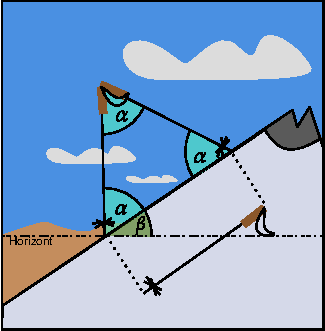
\includegraphics[width=\textwidth]{./Bilder/WinkelEinfacherFall.pdf}
  \end{minipage}%  
  \end{wrapfigure} Damit ist jeder Innenwinkel eines gleichseitigen Dreiecks 
  \begin{equation*}
   \frac{180^\circ}{3}=60^\circ\,.
  \end{equation*}
  Damit ist in dem rechten Bild Der Winkel $\alpha$ genau $60^\circ\,.$ Der Winkel $\beta$ ist unsere Hangneigung. Da wir den zweiten Stock hängen lassen und einmal von Windstille ausgehen, ist dieser Orthogonal auf dem Horizont. Damit ergänzen sich $\beta$ und $\alpha$ zu $90^\circ$ und somit ist $\beta=30^\circ\,.$

  \subsection*{Der Allgemeine Fall}
  Um die Faußtformel für belibige $l$ zu begründen benötigen wir zunächst einen Hilfssatz, d.h. ein sogenanntes Lemma:

  \begin{lemma}[Der Kosinussatz]~\\
\noindent
\begin{minipage}[t]{0.79\linewidth}
     In einem Dreieck $\Delta ABC$ mit Seitenlängen $a,b,c$ und der Winkelgröße $\alpha$ wie in der Abbildung rechts gilt, das Verhältnis
     \begin{equation*}
      b^2=a^2-c^2+2bc\cos(\alpha)\,.
     \end{equation*}
\end{minipage}% \hfill
\begin{minipage}[t]{0.19\linewidth}
\vspace{-5pt}

 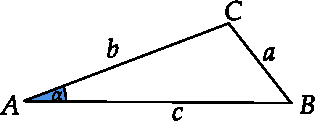
\includegraphics[width=\textwidth]{./Bilder/KosinussatzSetup.pdf}
\end{minipage}
  \end{lemma}
  
  \begin{proof}[Beweis]~ 
  \InsertBoxR{0}{\centering 
  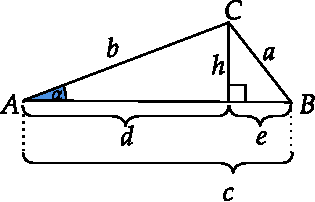
\includegraphics[width=0.3\linewidth]{./Bilder/KosinussatzSetupHöhe.pdf}
  } Wir starten, indem wir die Höhe auf die Seite $c$ errichten. Das heißt, wir errichten eine Orthogonale auf $c$ durch $C$. Der Fußpunkt der Höhe teilt die Seite $c$ in die beiden Teile $d$ und $e$. Somit gilt
  \begin{equation}
  	e=c-d\label{eq: d+e}
  \end{equation} Nun haben wir 2 rechtwinklige Dreiecke für die wie den Satz des Pythagoras anwenden können:
  \begin{align}
  	b^2&=h^2+d^2 \label{eq: SDP1}\\
  	a^2&=h^2+e^2~\Leftrightarrow h^2=a^2-e^2\label{eq: SDP2}\,.
  \end{align} Ersetzen wir nun damit das $h^2$ in der Gleichung (\ref{eq: SDP1}) erhalten wir
  \begin{equation*}
  	b^2=a^2-e^2+d^2\,.
  \end{equation*} Hier ersetzen wir nun das $e$ mittels Gleichung (\ref{eq: d+e}) und erhalten
  \begin{align*}
  	b^2&=a^2-(c-d)^2+d^2\\
  	&=a^2-(c^2+2cd+d^2)+d^2\\
  	&=a^2-c^2-2cd\\
  \end{align*} Jetzt wollen wir noch das $d$ loswerden. Dazu verwenden wir den Kosinus. Zur Erinnerung: Der Kosinus bildet in einem gleichschenkligen Dreieck einen Winkel auf das Verhältnis aus Ankathete und Hypothenuse. In unserem Dreieck bedeutet das für den Winkel $\alpha$: 
  \begin{equation*}
  	\cos(\alpha)=\frac{d}{b} ~\Leftrightarrow d=b \cos(\alpha)
  \end{equation*} Setzen wir das nun für $d$ ein so erhalten wir die gewollte Gleichung
  \begin{equation*}
  	b^2=a^2-c^2-2bc \cos(\alpha)
  \end{equation*}
   \end{proof}
   \par
   \begin{wrapfigure}{r}{0.42\textwidth}
   	\vspace{-\intextsep}
   	\centering
   	\begin{minipage}{0.39\textwidth}
   		\vspace{0pt}
   		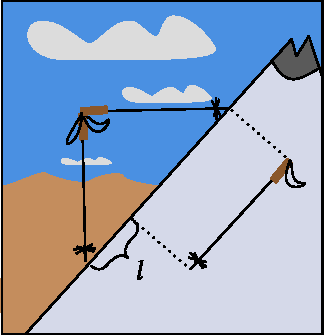
\includegraphics{./Bilder/AllgemeinerAufbau.pdf}
   		%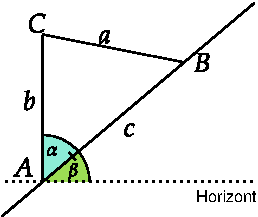
\includegraphics{./Bilder/DreieckAllgemeinerFall.pdf}
   	\end{minipage}%
   \end{wrapfigure}
   Geben wir nun dem entstehenden Dreieck die Bezeichnungen, welche rechts zu sehen sind. Dann gilt das $a$ und $b$ beide genau eine Skistocklänge ($SL$) betragen und $c$ eine Skistocklänge plus $l$, d.h. $c=1SL+l$. Da $\beta$ und $\alpha$ sich zu $90^\circ$ ergänzen gilt, $\beta=90^\circ-\alpha$ und mit dem Kosinussatz haben wir \begin{equation*}
   	\alpha=\cos^{-1}\left(\frac{b^2-a^2+c^2}{2bc}\right)
   \end{equation*}
Nun ist kürzt sich $b^2-a^2=0$ und wir erhalten 
\begin{equation*}
	\alpha=\cos{-1}\left(\frac{(SL+l)^2}{2SL(SL+l)}\right)
\end{equation*}